% Created 2020-09-01 二 18:26
% Intended LaTeX compiler: pdflatex
\documentclass[11pt]{article}
\usepackage[utf8]{inputenc}
\usepackage[T1]{fontenc}
\usepackage{graphicx}
\usepackage{grffile}
\usepackage{longtable}
\usepackage{wrapfig}
\usepackage{rotating}
\usepackage[normalem]{ulem}
\usepackage{amsmath}
\usepackage{textcomp}
\usepackage{amssymb}
\usepackage{capt-of}
\usepackage{hyperref}
\usepackage{minted}
%%%%%%%%%%%%%%%%%%%%%%%%%%%%%%%%%%%%%%
%% TIPS                                 %%
%%%%%%%%%%%%%%%%%%%%%%%%%%%%%%%%%%%%%%
% \substack{a\\b} for multiple lines text

\usepackage[utf8]{inputenc}

\usepackage[B1,T1]{fontenc}

% pdfplots will load xolor automatically without option
\usepackage[dvipsnames]{xcolor}
%%%%%%%%%%%%%%%%%%%%%%%%%%%%%%%%%%%%%%%
%% MATH related pacakge                  %%
%%%%%%%%%%%%%%%%%%%%%%%%%%%%%%%%%%%%%%%
% \usepackage{amsmath} mathtools loads the amsmath
\usepackage{amsmath}
\usepackage{mathtools}


\usepackage{amsthm}
\usepackage{amsbsy}

%\usepackage{commath}

\usepackage{amssymb}
\usepackage{mathrsfs}
%\usepackage{mathabx}
\usepackage{stmaryrd}
\usepackage{empheq}

\usepackage{scalerel}
\usepackage{stackengine}
\usepackage{stackrel}

\usepackage{nicematrix}
\usepackage{tensor}
\usepackage{blkarray}
\usepackage{siunitx}
\usepackage[f]{esvect}

\usepackage{unicode-math}
\setmainfont{TeX Gyre Pagella}
% \setmathfont{STIX}
% \setmathfont{texgyrepagella-math.otf}
% \setmathfont{Libertinus Math}
\setmathfont{Latin Modern Math}
\setmathfont[range={\mscra,\mscrb,\mscrc,\mscrd,\mscre,\mscrf,\mscrg,\mscrh,\mscri,\mscrj,\mscrk,\mscrl,\mscrm,\mscrn,\mscro,\mscrp,\mscrq,\mscrr,\mscrs,\mscrt,\mscru,\mscrv,\mscrw,\mscrx,\mscry,\mscrz,\mscrA,\mscrB,\mscrC,\mscrD,\mscrE,\mscrF,\mscrG,\mscrH,\mscrI,\mscrJ,\mscrK,\mscrL,\mscrM,\mscrN,\mscrO,\mscrP,\mscrQ,\mscrR,\mscrS,\mscrT,\mscrU,\mscrV,\mscrW,\mscrX,\mscrY,\mscrZ}]{Latin Modern Math}
\setmathfont[range={\smwhtdiamond,\enclosediamond,\varlrtriangle}]{Latin Modern Math}
\setmathfont[range={\rightrightarrows,\twoheadrightarrow,\leftrightsquigarrow,\triangledown}]{XITS Math}
\setmathfont[range={\int,\setminus}]{Libertinus Math}



%%%%%%%%%%%%%%%%%%%%%%%%%%%%%%%%%%%%%%%
%% TIKZ related packages                 %%
%%%%%%%%%%%%%%%%%%%%%%%%%%%%%%%%%%%%%%%

\usepackage{pgfplots}
\pgfplotsset{compat=1.15}
\usepackage{tikz}
\usepackage{tikz-cd}
\usepackage{tikz-qtree}

\usetikzlibrary{arrows,positioning,calc,fadings,decorations,matrix,decorations,shapes.misc}
%setting from geogebra
\definecolor{ccqqqq}{rgb}{0.8,0,0}


%%%%%%%%%%%%%%%%%%%%%%%%%%%%%%%%%%%%%%%
%% MISCLELLANEOUS packages               %%
%%%%%%%%%%%%%%%%%%%%%%%%%%%%%%%%%%%%%%%
\usepackage[most]{tcolorbox}
\usepackage{threeparttable}
\usepackage{tabularx}

\usepackage{enumitem}

% wrong with preview
\usepackage{subcaption}
\usepackage{caption}
% {\aunclfamily\Huge}
\usepackage{auncial}

\usepackage{float}

\usepackage{fancyhdr}

\usepackage{ifthen}
\usepackage{xargs}


\usepackage{imakeidx}
\usepackage{hyperref}
\usepackage{soul}


%\usepackage[xetex]{preview}
%%%%%%%%%%%%%%%%%%%%%%%%%%%%%%%%%%%%%%%
%% USEPACKAGES end                       %%
%%%%%%%%%%%%%%%%%%%%%%%%%%%%%%%%%%%%%%%

% \setlist{nosep}
% \numberwithin{equation}{subsection}
% \fancyhead{} % Clear the headers
% \renewcommand{\headrulewidth}{0pt} % Width of line at top of page
% \fancyhead[R]{\slshape\leftmark} % Mark right [R] of page with Chapter name [\leftmark]
% \pagestyle{fancy} % Set default style for all content pages (not TOC, etc)


% \newlength\shlength
% \newcommand\vect[2][0]{\setlength\shlength{#1pt}%
%   \stackengine{-5.6pt}{$#2$}{\smash{$\kern\shlength%
%     \stackengine{7.55pt}{$\mathchar"017E$}%
%       {\rule{\widthof{$#2$}}{.57pt}\kern.4pt}{O}{r}{F}{F}{L}\kern-\shlength$}}%
%       {O}{c}{F}{T}{S}}


\indexsetup{othercode=\small}
\makeindex[columns=2,options={-s /media/wu/file/stuuudy/notes/index_style.ist},intoc]
\makeatletter
\def\@idxitem{\par\hangindent 0pt}
\makeatother


%\newcounter{dummy} \numberwithin{dummy}{section}
\newtheorem{dummy}{dummy}[section]
\theoremstyle{definition}
\newtheorem{definition}[dummy]{Definition}
\theoremstyle{plain}
\newtheorem{corollary}[dummy]{Corollary}
\newtheorem{lemma}[dummy]{Lemma}
\newtheorem{proposition}[dummy]{Proposition}
\newtheorem{theorem}[dummy]{Theorem}
\theoremstyle{definition}
\newtheorem{examplle}{Example}[section]
\theoremstyle{remark}
\newtheorem*{remark}{Remark}
\newtheorem{exercise}{Exercise}[subsection]
\newtheorem{observation}{Observation}[section]


\newenvironment{claim}[1]{\par\noindent\textbf{Claim:}\space#1}{}

\makeatletter
\DeclareFontFamily{U}{tipa}{}
\DeclareFontShape{U}{tipa}{m}{n}{<->tipa10}{}
\newcommand{\arc@char}{{\usefont{U}{tipa}{m}{n}\symbol{62}}}%

\newcommand{\arc}[1]{\mathpalette\arc@arc{#1}}

\newcommand{\arc@arc}[2]{%
  \sbox0{$\m@th#1#2$}%
  \vbox{
    \hbox{\resizebox{\wd0}{\height}{\arc@char}}
    \nointerlineskip
    \box0
  }%
}
\makeatother

\setcounter{MaxMatrixCols}{20}
%%%%%%% ABS
\DeclarePairedDelimiter\abss{\lvert}{\rvert}%
\DeclarePairedDelimiter\normm{\lVert}{\rVert}%

% Swap the definition of \abs* and \norm*, so that \abs
% and \norm resizes the size of the brackets, and the
% starred version does not.
\makeatletter
\let\oldabs\abss
%\def\abs{\@ifstar{\oldabs}{\oldabs*}}
\newcommand{\abs}{\@ifstar{\oldabs}{\oldabs*}}
\newcommand{\norm}[1]{\left\lVert#1\right\rVert}
%\let\oldnorm\normm
%\def\norm{\@ifstar{\oldnorm}{\oldnorm*}}
%\renewcommand{norm}{\@ifstar{\oldnorm}{\oldnorm*}}
\makeatother

% \newcommand\what[1]{\ThisStyle{%
%     \setbox0=\hbox{$\SavedStyle#1$}%
%     \stackengine{-1.0\ht0+.5pt}{$\SavedStyle#1$}{%
%       \stretchto{\scaleto{\SavedStyle\mkern.15mu\char'136}{2.6\wd0}}{1.4\ht0}%
%     }{O}{c}{F}{T}{S}%
%   }
% }

% \newcommand\wtilde[1]{\ThisStyle{%
%     \setbox0=\hbox{$\SavedStyle#1$}%
%     \stackengine{-.1\LMpt}{$\SavedStyle#1$}{%
%       \stretchto{\scaleto{\SavedStyle\mkern.2mu\AC}{.5150\wd0}}{.6\ht0}%
%     }{O}{c}{F}{T}{S}%
%   }
% }

% \newcommand\wbar[1]{\ThisStyle{%
%     \setbox0=\hbox{$\SavedStyle#1$}%
%     \stackengine{.5pt+\LMpt}{$\SavedStyle#1$}{%
%       \rule{\wd0}{\dimexpr.3\LMpt+.3pt}%
%     }{O}{c}{F}{T}{S}%
%   }
% }

\newcommand{\bl}[1] {\boldsymbol{#1}}
\newcommand{\Wt}[1] {\stackrel{\sim}{\smash{#1}\rule{0pt}{1.1ex}}}
\newcommand{\wt}[1] {\widetilde{#1}}
\newcommand{\tf}[1] {\textbf{#1}}


%For boxed texts in align, use Aboxed{}
%otherwise use boxed{}

\DeclareMathSymbol{\widehatsym}{\mathord}{largesymbols}{"62}
\newcommand\lowerwidehatsym{%
  \text{\smash{\raisebox{-1.3ex}{%
    $\widehatsym$}}}}
\newcommand\fixwidehat[1]{%
  \mathchoice
    {\accentset{\displaystyle\lowerwidehatsym}{#1}}
    {\accentset{\textstyle\lowerwidehatsym}{#1}}
    {\accentset{\scriptstyle\lowerwidehatsym}{#1}}
    {\accentset{\scriptscriptstyle\lowerwidehatsym}{#1}}
  }


\newcommand{\cupdot}{\mathbin{\dot{\cup}}}
\newcommand{\bigcupdot}{\mathop{\dot{\bigcup}}}

\usepackage{graphicx}

\usepackage[toc,page]{appendix}

% text on arrow for xRightarrow
\makeatletter
%\newcommand{\xRightarrow}[2][]{\ext@arrow 0359\Rightarrowfill@{#1}{#2}}
\makeatother

% Arbitrary long arrow
\newcommand{\Rarrow}[1]{%
\parbox{#1}{\tikz{\draw[->](0,0)--(#1,0);}}
}

\newcommand{\LRarrow}[1]{%
\parbox{#1}{\tikz{\draw[<->](0,0)--(#1,0);}}
}


\makeatletter
\providecommand*{\rmodels}{%
  \mathrel{%
    \mathpalette\@rmodels\models
  }%
}
\newcommand*{\@rmodels}[2]{%
  \reflectbox{$\m@th#1#2$}%
}
\makeatother







\newcommand{\trcl}[1]{%
  \mathrm{trcl}{(#1)}
}



% Roman numerals
\makeatletter
\newcommand*{\rom}[1]{\expandafter\@slowromancap\romannumeral #1@}
\makeatother
% \\def \\b\([a-zA-Z]\) {\\boldsymbol{[a-zA-z]}}
% \\DeclareMathOperator{\\b\1}{\\textbf{\1}}


\DeclareMathOperator{\bx}{\textbf{x}}
\DeclareMathOperator{\bz}{\textbf{z}}
\DeclareMathOperator{\bff}{\textbf{f}}
\DeclareMathOperator{\ba}{\textbf{a}}
\DeclareMathOperator{\bk}{\textbf{k}}
\DeclareMathOperator{\bs}{\textbf{s}}
\DeclareMathOperator{\bh}{\textbf{h}}
\DeclareMathOperator{\bc}{\textbf{c}}
\DeclareMathOperator{\br}{\textbf{r}}
\DeclareMathOperator{\bi}{\textbf{i}}
\DeclareMathOperator{\bj}{\textbf{j}}
\DeclareMathOperator{\bn}{\textbf{n}}
\DeclareMathOperator{\be}{\textbf{e}}
\DeclareMathOperator{\bo}{\textbf{o}}
\DeclareMathOperator{\bU}{\textbf{U}}
\DeclareMathOperator{\bL}{\textbf{L}}
\DeclareMathOperator{\bV}{\textbf{V}}
\def \bzero {\mathbf{0}}
\def \btwo {\mathbf{2}}
\DeclareMathOperator{\bv}{\textbf{v}}
\DeclareMathOperator{\bp}{\textbf{p}}
\DeclareMathOperator{\bI}{\textbf{I}}
\DeclareMathOperator{\bM}{\textbf{M}}
\DeclareMathOperator{\bN}{\textbf{N}}
\DeclareMathOperator{\bK}{\textbf{K}}
\DeclareMathOperator{\bt}{\textbf{t}}
\DeclareMathOperator{\bb}{\textbf{b}}
\DeclareMathOperator{\bA}{\textbf{A}}
\DeclareMathOperator{\bX}{\textbf{X}}
\DeclareMathOperator{\bu}{\textbf{u}}
\DeclareMathOperator{\bS}{\textbf{S}}
\DeclareMathOperator{\bZ}{\textbf{Z}}
\DeclareMathOperator{\by}{\textbf{y}}
\DeclareMathOperator{\bw}{\textbf{w}}
\DeclareMathOperator{\bT}{\textbf{T}}
\DeclareMathOperator{\bF}{\textbf{F}}
\DeclareMathOperator{\bmm}{\textbf{m}}
\DeclareMathOperator{\bW}{\textbf{W}}
\DeclareMathOperator{\bR}{\textbf{R}}
\DeclareMathOperator{\bC}{\textbf{C}}
\DeclareMathOperator{\bD}{\textbf{D}}
\DeclareMathOperator{\bE}{\textbf{E}}
\DeclareMathOperator{\bQ}{\textbf{Q}}
\DeclareMathOperator{\bP}{\textbf{P}}
\DeclareMathOperator{\bY}{\textbf{Y}}
\DeclareMathOperator{\bH}{\textbf{H}}
\DeclareMathOperator{\bB}{\textbf{B}}
\DeclareMathOperator{\bG}{\textbf{G}}
\def \blambda {\symbf{\lambda}}
\def \boldeta {\symbf{\eta}}
\def \balpha {\symbf{\alpha}}
\def \bbeta {\symbf{\beta}}
\def \bgamma {\symbf{\gamma}}
\def \bxi {\symbf{\xi}}
\def \bLambda {\symbf{\Lambda}}

\newcommand{\bto}{{\boldsymbol{\to}}}
\newcommand{\Ra}{\Rightarrow}
\newcommand\und[1]{\underline{#1}}
\def \bPhi {\boldsymbol{\Phi}}
\def \btheta {\boldsymbol{\theta}}
\def \bTheta {\boldsymbol{\Theta}}
\def \bmu {\boldsymbol{\mu}}
\def \bphi {\boldsymbol{\phi}}
\def \bSigma {\boldsymbol{\Sigma}}
\def \lb {\left\{}
\def \rb {\right\}}
\def \la {\langle}
\def \ra {\rangle}
\def \caln {\mathcal{N}}
\def \dissum {\displaystyle\Sigma}
\def \dispro {\displaystyle\prod}
\def \E {\mathbb{E}}
\def \Q {\mathbb{Q}}
\def \N {\mathbb{N}}
\def \V {\mathbb{V}}
\def \R {\mathbb{R}}
\def \P {\mathbb{P}}
\def \A {\mathbb{A}}
\def \F {\mathbb{F}}
\def \Z {\mathbb{Z}}
\def \I {\mathbb{I}}
\def \C {\mathbb{C}}
\def \cala {\mathcal{A}}
\def \cale {\mathcal{E}}
\def \calb {\mathcal{B}}
\def \calq {\mathcal{Q}}
\def \calp {\mathcal{P}}
\def \cals {\mathcal{S}}
\def \calx {\mathcal{X}}
\def \caly {\mathcal{Y}}
\def \calg {\mathcal{G}}
\def \cald {\mathcal{D}}
\def \caln {\mathcal{N}}
\def \calr {\mathcal{R}}
\def \calt {\mathcal{T}}
\def \calm {\mathcal{M}}
\def \calw {\mathcal{W}}
\def \calc {\mathcal{C}}
\def \calv {\mathcal{V}}
\def \calf {\mathcal{F}}
\def \calk {\mathcal{K}}
\def \call {\mathcal{L}}
\def \calu {\mathcal{U}}
\def \calo {\mathcal{O}}
\def \calh {\mathcal{H}}
\def \cali {\mathcal{I}}

\def \bcup {\bigcup}

% set theory

\def \zfcc {\textbf{ZFC}^-}
\def \ac  {\textbf{AC}}
\def \gl  {\textbf{L }}
\def \gll {\textbf{L}}
\newcommand{\zfm}{$\textbf{ZF}^-$}

%\def \zfm {$\textbf{ZF}^-$}
\def \zfmm {\textbf{ZF}^-}
\def \wf {\textbf{WF }}
\def \on {\textbf{On }}
\def \cm {\textbf{M }}
\def \cn {\textbf{N }}
\def \cv {\textbf{V }}
\def \zc {\textbf{ZC }}
\def \zcm {\textbf{ZC}}
\def \zff {\textbf{ZF}}
\def \wfm {\textbf{WF}}
\def \onm {\textbf{On}}
\def \cmm {\textbf{M}}
\def \cnm {\textbf{N}}
\def \cvm {\textbf{V}}
\def \gchh {\textbf{GCH}}
\renewcommand{\restriction}{\mathord{\upharpoonright}}
\def \pred {\text{pred}}

\def \rank {\text{rank}}
\def \con {\text{Con}}
\def \deff {\text{Def}}


\def \uin {\underline{\in}}
\def \oin {\overline{\in}}
\def \uR {\underline{R}}
\def \oR {\overline{R}}
\def \uP {\underline{P}}
\def \oP {\overline{P}}

\def \Ra {\Rightarrow}

\def \e {\enspace}

\def \sgn {\operatorname{sgn}}
\def \gen {\operatorname{gen}}
\def \Hom {\operatorname{Hom}}
\def \hom {\operatorname{hom}}
\def \Sub {\operatorname{Sub}}

\def \supp {\operatorname{supp}}

\def \epiarrow {\twoheadarrow}
\def \monoarrow {\rightarrowtail}
\def \rrarrow {\rightrightarrows}

% \def \minus {\text{-}}
% \newcommand{\minus}{\scalebox{0.75}[1.0]{$-$}}
% \DeclareUnicodeCharacter{002D}{\minus}


\def \tril {\triangleleft}

\def \ACF {\text{ACF}}
\def \GL {\text{GL}}
\def \PGL {\text{PGL}}
\def \equal {=}
\def \deg {\text{deg}}
\def \degree {\text{degree}}
\def \app {\text{App}}
\def \FV {\text{FV}}
\def \conv {\text{conv}}
\def \cont {\text{cont}}
\DeclareMathOperator{\cl}{\textbf{CL}}
\DeclareMathOperator{\sg}{sg}
\DeclareMathOperator{\trdeg}{trdeg}
\def \Ord {\text{Ord}}

\DeclareMathOperator{\cf}{cf}
\DeclareMathOperator{\zfc}{ZFC}

%\DeclareMathOperator{\Th}{Th}
%\def \th {\text{Th}}
% \newcommand{\th}{\text{Th}}
\DeclareMathOperator{\type}{type}
\DeclareMathOperator{\zf}{\textbf{ZF}}
\def \fa {\mathfrak{a}}
\def \fb {\mathfrak{b}}
\def \fc {\mathfrak{c}}
\def \fd {\mathfrak{d}}
\def \fe {\mathfrak{e}}
\def \ff {\mathfrak{f}}
\def \fg {\mathfrak{g}}
\def \fh {\mathfrak{h}}
%\def \fi {\mathfrak{i}}
\def \fj {\mathfrak{j}}
\def \fk {\mathfrak{k}}
\def \fl {\mathfrak{l}}
\def \fm {\mathfrak{m}}
\def \fn {\mathfrak{n}}
\def \fo {\mathfrak{o}}
\def \fp {\mathfrak{p}}
\def \fq {\mathfrak{q}}
\def \fr {\mathfrak{r}}
\def \fs {\mathfrak{s}}
\def \ft {\mathfrak{t}}
\def \fu {\mathfrak{u}}
\def \fv {\mathfrak{v}}
\def \fw {\mathfrak{w}}
\def \fx {\mathfrak{x}}
\def \fy {\mathfrak{y}}
\def \fz {\mathfrak{z}}
\def \fA {\mathfrak{A}}
\def \fB {\mathfrak{B}}
\def \fC {\mathfrak{C}}
\def \fD {\mathfrak{D}}
\def \fE {\mathfrak{E}}
\def \fF {\mathfrak{F}}
\def \fG {\mathfrak{G}}
\def \fH {\mathfrak{H}}
\def \fI {\mathfrak{I}}
\def \fJ {\mathfrak{J}}
\def \fK {\mathfrak{K}}
\def \fL {\mathfrak{L}}
\def \fM {\mathfrak{M}}
\def \fN {\mathfrak{N}}
\def \fO {\mathfrak{O}}
\def \fP {\mathfrak{P}}
\def \fQ {\mathfrak{Q}}
\def \fR {\mathfrak{R}}
\def \fS {\mathfrak{S}}
\def \fT {\mathfrak{T}}
\def \fU {\mathfrak{U}}
\def \fV {\mathfrak{V}}
\def \fW {\mathfrak{W}}
\def \fX {\mathfrak{X}}
\def \fY {\mathfrak{Y}}
\def \fZ {\mathfrak{Z}}

\def \sfA {\textsf{A}}
\def \sfB {\textsf{B}}
\def \sfC {\textsf{C}}
\def \sfD {\textsf{D}}
\def \sfE {\textsf{E}}
\def \sfF {\textsf{F}}
\def \sfG {\textsf{G}}
\def \sfH {\textsf{H}}
\def \sfI {\textsf{I}}
\def \sfj {\textsf{J}}
\def \sfK {\textsf{K}}
\def \sfL {\textsf{L}}
\def \sfM {\textsf{M}}
\def \sfN {\textsf{N}}
\def \sfO {\textsf{O}}
\def \sfP {\textsf{P}}
\def \sfQ {\textsf{Q}}
\def \sfR {\textsf{R}}
\def \sfS {\textsf{S}}
\def \sfT {\textsf{T}}
\def \sfU {\textsf{U}}
\def \sfV {\textsf{V}}
\def \sfW {\textsf{W}}
\def \sfX {\textsf{X}}
\def \sfY {\textsf{Y}}
\def \sfZ {\textsf{Z}}
\def \sfa {\textsf{a}}
\def \sfb {\textsf{b}}
\def \sfc {\textsf{c}}
\def \sfd {\textsf{d}}
\def \sfe {\textsf{e}}
\def \sff {\textsf{f}}
\def \sfg {\textsf{g}}
\def \sfh {\textsf{h}}
\def \sfi {\textsf{i}}
\def \sfj {\textsf{j}}
\def \sfk {\textsf{k}}
\def \sfl {\textsf{l}}
\def \sfm {\textsf{m}}
\def \sfn {\textsf{n}}
\def \sfo {\textsf{o}}
\def \sfp {\textsf{p}}
\def \sfq {\textsf{q}}
\def \sfr {\textsf{r}}
\def \sfs {\textsf{s}}
\def \sft {\textsf{t}}
\def \sfu {\textsf{u}}
\def \sfv {\textsf{v}}
\def \sfw {\textsf{w}}
\def \sfx {\textsf{x}}
\def \sfy {\textsf{y}}
\def \sfz {\textsf{z}}



%\DeclareMathOperator{\ker}{ker}
\DeclareMathOperator{\im}{im}

\DeclareMathOperator{\inn}{Inn}
\DeclareMathOperator{\AC}{\textbf{AC}}
\DeclareMathOperator{\cod}{cod}
\DeclareMathOperator{\dom}{dom}
\DeclareMathOperator{\ran}{ran}
\DeclareMathOperator{\textd}{d}
\DeclareMathOperator{\td}{d}
\DeclareMathOperator{\id}{id}
\DeclareMathOperator{\LT}{LT}
\DeclareMathOperator{\Mat}{Mat}
\DeclareMathOperator{\Eq}{Eq}
\DeclareMathOperator{\irr}{irr}
\DeclareMathOperator{\Fr}{Fr}
\DeclareMathOperator{\Gal}{Gal}
\DeclareMathOperator{\lcm}{lcm}
\DeclareMathOperator{\alg}{\text{alg}}
\DeclareMathOperator{\Th}{Th}

\DeclareMathOperator{\DAG}{DAG}
\DeclareMathOperator{\ODAG}{ODAG}

% \varprod
\DeclareSymbolFont{largesymbolsA}{U}{txexa}{m}{n}
\DeclareMathSymbol{\varprod}{\mathop}{largesymbolsA}{16}
% \DeclareMathSymbol{\tonm}{\boldsymbol{\to}\textbf{Nm}}
\def \tonm {\bto\textbf{Nm}}
\def \tohm {\bto\textbf{Hm}}

% Category theory
\DeclareMathOperator{\Ab}{\textbf{Ab}}
\DeclareMathOperator{\Alg}{\textbf{Alg}}
\DeclareMathOperator{\Rng}{\textbf{Rng}}
\DeclareMathOperator{\Sets}{\textbf{Sets}}
\DeclareMathOperator{\Met}{\textbf{Met}}
\DeclareMathOperator{\Aut}{\textbf{Aut}}
\DeclareMathOperator{\RMod}{R-\textbf{Mod}}
\DeclareMathOperator{\RAlg}{R-\textbf{Alg}}
\DeclareMathOperator{\LF}{LF}
\DeclareMathOperator{\op}{op}
% Model theory
\DeclareMathOperator{\tp}{tp}
\DeclareMathOperator{\Diag}{Diag}
\DeclareMathOperator{\el}{el}
\DeclareMathOperator{\depth}{depth}
\DeclareMathOperator{\FO}{FO}
\DeclareMathOperator{\fin}{fin}
\DeclareMathOperator{\qr}{qr}
\DeclareMathOperator{\Mod}{Mod}
\DeclareMathOperator{\TC}{TC}
\DeclareMathOperator{\KH}{KH}
\DeclareMathOperator{\Part}{Part}
\DeclareMathOperator{\Infset}{\textsf{Infset}}
\DeclareMathOperator{\DLO}{\textsf{DLO}}
\DeclareMathOperator{\sfMod}{\textsf{Mod}}
\DeclareMathOperator{\AbG}{\textsf{AbG}}
\DeclareMathOperator{\sfACF}{\textsf{ACF}}
% Computability Theorem
\DeclareMathOperator{\Tot}{Tot}
\DeclareMathOperator{\graph}{graph}
\DeclareMathOperator{\Fin}{Fin}
\DeclareMathOperator{\Cof}{Cof}
\DeclareMathOperator{\lh}{lh}
% Commutative Algebra
\DeclareMathOperator{\ord}{ord}
\DeclareMathOperator{\Idem}{Idem}
\DeclareMathOperator{\zdiv}{z.div}
\DeclareMathOperator{\Frac}{Frac}
\DeclareMathOperator{\rad}{rad}
\DeclareMathOperator{\nil}{nil}
\DeclareMathOperator{\Ann}{Ann}
\DeclareMathOperator{\End}{End}
\DeclareMathOperator{\coim}{coim}
\DeclareMathOperator{\coker}{coker}
\DeclareMathOperator{\Bil}{Bil}
\DeclareMathOperator{\Tril}{Tril}
% Topology
\newcommand{\interior}[1]{%
  {\kern0pt#1}^{\mathrm{o}}%
}

% \makeatletter
% \newcommand{\vect}[1]{%
%   \vbox{\m@th \ialign {##\crcr
%   \vectfill\crcr\noalign{\kern-\p@ \nointerlineskip}
%   $\hfil\displaystyle{#1}\hfil$\crcr}}}
% \def\vectfill{%
%   $\m@th\smash-\mkern-7mu%
%   \cleaders\hbox{$\mkern-2mu\smash-\mkern-2mu$}\hfill
%   \mkern-7mu\raisebox{-3.81pt}[\p@][\p@]{$\mathord\mathchar"017E$}$}

% \newcommand{\amsvect}{%
%   \mathpalette {\overarrow@\vectfill@}}
% \def\vectfill@{\arrowfill@\relbar\relbar{\raisebox{-3.81pt}[\p@][\p@]{$\mathord\mathchar"017E$}}}

% \newcommand{\amsvectb}{%
% \newcommand{\vect}{%
%   \mathpalette {\overarrow@\vectfillb@}}
% \newcommand{\vecbar}{%
%   \scalebox{0.8}{$\relbar$}}
% \def\vectfillb@{\arrowfill@\vecbar\vecbar{\raisebox{-4.35pt}[\p@][\p@]{$\mathord\mathchar"017E$}}}
% \makeatother
% \bigtimes

\DeclareFontFamily{U}{mathx}{\hyphenchar\font45}
\DeclareFontShape{U}{mathx}{m}{n}{
      <5> <6> <7> <8> <9> <10>
      <10.95> <12> <14.4> <17.28> <20.74> <24.88>
      mathx10
      }{}
\DeclareSymbolFont{mathx}{U}{mathx}{m}{n}
\DeclareMathSymbol{\bigtimes}{1}{mathx}{"91}
% \odiv
\DeclareFontFamily{U}{matha}{\hyphenchar\font45}
\DeclareFontShape{U}{matha}{m}{n}{
      <5> <6> <7> <8> <9> <10> gen * matha
      <10.95> matha10 <12> <14.4> <17.28> <20.74> <24.88> matha12
      }{}
\DeclareSymbolFont{matha}{U}{matha}{m}{n}
\DeclareMathSymbol{\odiv}         {2}{matha}{"63}


\newcommand\subsetsim{\mathrel{%
  \ooalign{\raise0.2ex\hbox{\scalebox{0.9}{$\subset$}}\cr\hidewidth\raise-0.85ex\hbox{\scalebox{0.9}{$\sim$}}\hidewidth\cr}}}
\newcommand\simsubset{\mathrel{%
  \ooalign{\raise-0.2ex\hbox{\scalebox{0.9}{$\subset$}}\cr\hidewidth\raise0.75ex\hbox{\scalebox{0.9}{$\sim$}}\hidewidth\cr}}}

\newcommand\simsubsetsim{\mathrel{%
  \ooalign{\raise0ex\hbox{\scalebox{0.8}{$\subset$}}\cr\hidewidth\raise1ex\hbox{\scalebox{0.75}{$\sim$}}\hidewidth\cr\raise-0.95ex\hbox{\scalebox{0.8}{$\sim$}}\cr\hidewidth}}}
\newcommand{\stcomp}[1]{{#1}^{\mathsf{c}}}

\setlength{\baselineskip}{0.8in}

\stackMath
\newcommand\yrightarrow[2][]{\mathrel{%
  \setbox2=\hbox{\stackon{\scriptstyle#1}{\scriptstyle#2}}%
  \stackunder[0pt]{%
    \xrightarrow{\makebox[\dimexpr\wd2\relax]{$\scriptstyle#2$}}%
  }{%
   \scriptstyle#1\,%
  }%
}}
\newcommand\yleftarrow[2][]{\mathrel{%
  \setbox2=\hbox{\stackon{\scriptstyle#1}{\scriptstyle#2}}%
  \stackunder[0pt]{%
    \xleftarrow{\makebox[\dimexpr\wd2\relax]{$\scriptstyle#2$}}%
  }{%
   \scriptstyle#1\,%
  }%
}}
\newcommand\yRightarrow[2][]{\mathrel{%
  \setbox2=\hbox{\stackon{\scriptstyle#1}{\scriptstyle#2}}%
  \stackunder[0pt]{%
    \xRightarrow{\makebox[\dimexpr\wd2\relax]{$\scriptstyle#2$}}%
  }{%
   \scriptstyle#1\,%
  }%
}}
\newcommand\yLeftarrow[2][]{\mathrel{%
  \setbox2=\hbox{\stackon{\scriptstyle#1}{\scriptstyle#2}}%
  \stackunder[0pt]{%
    \xLeftarrow{\makebox[\dimexpr\wd2\relax]{$\scriptstyle#2$}}%
  }{%
   \scriptstyle#1\,%
  }%
}}

\newcommand\altxrightarrow[2][0pt]{\mathrel{\ensurestackMath{\stackengine%
  {\dimexpr#1-7.5pt}{\xrightarrow{\phantom{#2}}}{\scriptstyle\!#2\,}%
  {O}{c}{F}{F}{S}}}}
\newcommand\altxleftarrow[2][0pt]{\mathrel{\ensurestackMath{\stackengine%
  {\dimexpr#1-7.5pt}{\xleftarrow{\phantom{#2}}}{\scriptstyle\!#2\,}%
  {O}{c}{F}{F}{S}}}}

\newenvironment{bsm}{% % short for 'bracketed small matrix'
  \left[ \begin{smallmatrix} }{%
  \end{smallmatrix} \right]}

\newenvironment{psm}{% % short for ' small matrix'
  \left( \begin{smallmatrix} }{%
  \end{smallmatrix} \right)}

\newcommand{\bbar}[1]{\mkern 1.5mu\overline{\mkern-1.5mu#1\mkern-1.5mu}\mkern 1.5mu}

\newcommand{\bigzero}{\mbox{\normalfont\Large\bfseries 0}}
\newcommand{\rvline}{\hspace*{-\arraycolsep}\vline\hspace*{-\arraycolsep}}

\font\zallman=Zallman at 40pt
\font\elzevier=Elzevier at 40pt

\newcommand\isoto{\stackrel{\textstyle\sim}{\smash{\longrightarrow}\rule{0pt}{0.4ex}}}
\newcommand\embto{\stackrel{\textstyle\prec}{\smash{\longrightarrow}\rule{0pt}{0.4ex}}}
\usepackage[UTF8]{ctex}
\author{Qi'ao Chen}
\date{\today}
\title{10天入门高数}
\hypersetup{
 pdfauthor={Qi'ao Chen},
 pdftitle={10天入门高数},
 pdfkeywords={},
 pdfsubject={},
 pdfcreator={Emacs 26.3 (Org mode 9.4)}, 
 pdflang={English}}
\begin{document}

\maketitle
\tableofcontents \clearpage
\section{函数与极限}
\label{sec:org6c69452}
\subsection{映射与函数}
\label{sec:org28238f0}
\begin{proposition}[]
Suppose \(f(x)\)'s domain is \((-l,l)\), then there is odd function
\(f_o(x)\) and even function \(f_e(x)\) on \((-l,l)\) s.t.
\begin{equation*}
f(x)=g(x)+h(x)
\end{equation*}
\end{proposition}

\begin{proof}
\begin{equation*}
f_e(x)=\frac{f(x)+f(-x)}{2}\quad
f_o(x)=\frac{f(x)-f(-x)}{x}
\end{equation*}
\end{proof}

基本初等函数
\begin{itemize}
\item 幂函数: \(y=x^\mu\) (\(\mu\in\R\) is a constant)
\item 指数函数:\(y=a^x\) (\(a\iffalse<\fi>0\) and \(a\neq1\))
\item 对数函数:\(y=\log_ax\) (\(a>0\) and \(a\neq1\))
\item 三角函数:\(y=\sin x,\cos x,\tan x\)
\item 反三角函数:\(y=\arcsin x,\arccos x,\arctan x\)
\end{itemize}
\subsection{数列的极限}
\label{sec:org1900f15}
\begin{definition}[]
suppose \(\{x_n\}\) is a sequence, if there is a constant \(a\) for any
positive \(\epsilon\), there is a positive integer \(N\) s..t if \(n>N\), then
\begin{equation*}
\abs{x_n-a}<\epsilon
\end{equation*}
always holds, then \(a\) is called the limit of \(\{x_n\}\), or \(\{x_n\}\)
converges to \(a\), written as
\begin{equation*}
\lim_{n\to\infty}x_n=a
\end{equation*}
or
\begin{equation*}
x_n\to a(n\to \infty)
\end{equation*}
\end{definition}

\begin{theorem}[极限的唯一性]
如果数列\(\{x_n\}\)收敛,那么它的极限唯一
\end{theorem}

\begin{proof}
假设同时有\(x_n\to a\)及\(x_n\to b\),且\(a<b\),取\(\epsilon=\frac{b-a}{2}\),
因为\(\lim_{n\to\infty}x_n=a\),故存在正整数\(N_1\),当\(n>N_1\)时,
\begin{equation}
\abs{x_n-a}<\frac{b-a}{2}\label{eq2-2}
\end{equation}
同理有当\(n>N_2\)时
\begin{equation}
\abs{x_n-b}<\frac{b-a}{2}\label{eq2-3}
\end{equation}
取\(N=\max\{N_1,N_2\}\),由\eqref{eq2-2} 有\(x_n<\frac{a+b}{2}\),由
\eqref{eq2-3} 有\(x_n>\frac{a+b}{2}\),矛盾
\end{proof}

\begin{theorem}[收敛数列的有界性]
如果数列\(\{x_n\}\)收敛,那么数列\(\{x_n\}\)一定有界
\end{theorem}

\begin{proof}
因为数列\(\{x_n\}\)收敛,设\(\lim_{n\to\infty}x_n=a\),对于\(\epsilon=1\),存
在正整数\(N\),当\(n>N\)时有
\begin{equation*}
\abs{x_n-a}<1
\end{equation*}
于是当\(n>N\)时
\begin{equation*}
\abs{x_n}=\abs{x_n-a+a}\le\abs{x_n-a}+\abs{a}<1+\abs{a}
\end{equation*}
取\(M=\max\{\abs{x_1},\dots,\abs{x_N},1+\abs{a}\}\),那么数列\(\{x_n\}\)中的
一切\(x_n\)都满足不等式
\begin{equation*}
\abs{x_n}\le M
\end{equation*}
\end{proof}

\begin{theorem}[收敛数列的保号性]
如果\(\lim_{n\to\infty}x_n=a\)且\(a>0\)(或\(a<0\)),那么存在正整数\(N\),当
\(n>N\)时,都有\(x_n>0\)(或\(x_n<0\))
\end{theorem}

\begin{proof}
Suppose \(a>0\), let \(\epsilon=\frac{a}{2}>0\), then there is \(N\) for
\(n>N\) s.t.
\begin{equation*}
\abs{x_n-a}<\frac{a}{2}
\end{equation*}
Hence
\begin{equation*}
x_n>a-\frac{a}{2}=\frac{a}{2}>0
\end{equation*}
\end{proof}

\begin{corollary}[]
如果数列\(\{x_n\}\)从某项起有\(x_n\ge0\)(或\(x_n\le0\)),且
\(\lim_{n\to\infty}x_n=a\),那么\(a\ge0\)(或\(a\le0\))
\end{corollary}

在数列\(\{x_n\}\)中任意抽取无限多项并保持这些项在原数列\(\{x_n\}\)中的先后次
序,这样得到的一个数列称为原数列\(\{x_n\}\)的 \textbf{子数列}

\begin{theorem}[收敛数列与其子数列的关系]
如果数列\(\{x_n\}\)收敛于\(a\),那么它的任一子数列也收敛,且极限也是\(a\)
\end{theorem}

\begin{proof}
设数列\(\{x_{n_k}\}\)是数列\(\{x_n\}\)的任一子数列

由于\(\lim_{n\to\infty}x_n=a\),故对任意\(\epsilon>0\),存在正整数\(N\)当\(n>N\)时,
\(\abs{x_n-a}<\epsilon\)

取\(K=N\),则当\(k>K\)时,\(n_k>n_K=n_N\ge N\),于是
\(\abs{x_{n_k}-a}<\epsilon\),因此\(\lim_{k\to\infty}x_{n_k}=a\)
\end{proof}
\subsection{函数的极限}
\label{sec:org960cb1f}
\subsubsection{函数极限的定义}
\label{sec:orgbb84f0d}
\begin{definition}[]
设函数\(f(x)\)在点\(x_0\)的某一去心邻域内有定义,如果存在常数\(A\)对于任一给
定的正数 \(\epsilon\) 总存在正数 \(\delta\) 使得当\(x\) 满足不等式\(0<\abs{x-x_0}<\delta\)时,对
应的函数值 \(f(x)\) 都满足不等式
\begin{equation*}
\abs{f(x)-A}<\epsilon
\end{equation*}
那么常数\(A\)就叫做 \textbf{函数\(f(x)\)当\(x\to x_0\)时的极限} ,记作
\begin{equation*}
\lim_{x\to x_0}f(x)=A \quad\text{ or }\quad
f(x)\to A(\text{when }x\to x_0)
\end{equation*}
\end{definition}

\begin{proposition}[]
\(\lim_{x\to1}(2x-1)=1\)
\end{proposition}

\begin{proof}
Since
\begin{equation*}
\abs{f(x)-A}=\abs{2x-2}=2\abs{x-1}
\end{equation*}
for any \(\epsilon>0\), let \(\delta=\epsilon/2\), then if
\begin{equation*}
0<\abs{x-1}<\delta
\end{equation*}
we have
\begin{equation*}
\abs{f(x)-1}=2\abs{x-1}<\epsilon
\end{equation*}
hence
\begin{equation*}
\lim_{x\to1}(2x-1)=1
\end{equation*}
\end{proof}

将\(0<\abs{x-x_0}<\delta\) 改为\(x_0-\delta<x<x_0\),那么\(A\)就叫做函数
\(f(x)\) 当\(x\to x_0\)时的 \textbf{左极限} ,记作
\begin{equation*}
\lim_{x\to x_0^-}f(x)=A\quad\text{ or }\quad
f(x_0^-)=A
\end{equation*}

函数\(f(x)\)当\(x\to x_0\)时极限存在的充分必要条件时左极限及右极限各自存在且
相等

\begin{definition}[]
设函数\(f(x)\)当\(\abs{x}\)大于某一正数时有定义,如果存在常数\(A\)对于任意给定
的正数 \(\epsilon\) 总存在正数 \(X\) 使得当 \(x\) 满足不等式  \(\abs{x}>X\) 时,对应的函
数值满足
\begin{equation*}
\abs{f(x)-A}<\epsilon
\end{equation*}
那么常数 \(A\) 就叫做 \textbf{函数\(f(x)\)当\(x\to\infty\)时的极限} ,记作
\begin{equation*}
\lim_{x\to\infty}f(x)=A \quad\text{ or }\quad
f(x)\to A(\text{when }x\to\infty)
\end{equation*}
\end{definition}
\subsubsection{函数极限的性质}
\label{sec:org1386f06}
\begin{theorem}[函数极限的唯一性]
如果\(\lim_{x\to x_0}f(x)\)存在,那么这极限唯一
\end{theorem}

\begin{proof}
If \(\lim_{x\to x_0}f(x)=a\) and \(\lim_{x\to x_0}f(x)=b\), let
\(\epsilon=\frac{b-a}{2}\), there is \(\delta_1\) and \(\delta_2\) s.t. for
\(0<\abs{x-x_0}<\delta_1\), \(\abs{f(x)-a}<\frac{b-a}{2}\), and balabala\ldots{}
\end{proof}

\begin{theorem}[函数极限的局部有界性]
如果\(\lim_{x\to x_0}f(x)=A\),那么存在常数\(M>0\)和\(\delta>0\)使得当
\(0<\abs{x-x_0}<\delta\)时,有\(\abs{f(x)}\le M\)
\end{theorem}

\begin{proof}
取\(\epsilon=1\), then there is \(\delta\) for \(0<\abs{x-x_0}<\delta\), we have
\begin{equation*}
\abs{f(x)-A}<1\Rightarrow\abs{f(x)}\le\abs{f(x)-A}+\abs{A}<\abs{A}+1
\end{equation*}
记\(M=\abs{A}+1\)
\end{proof}

\begin{theorem}[函数极限的局部保号性]
如果\(\lim_{x\to x_0}f(x)=A\),且\(A>0\)(或\(A<0\)),那么存在常数\(\delta>0\),使得
当\(0<\abs{x-x_0}<\delta\)时有\(f(x)>0\) (或\(f(x)<0\))
\end{theorem}
\subsection{无穷大与无穷小}
\label{sec:org1fb2184}
\begin{definition}[]
如果函数\(f(x)\)当\(x\to x_0\)(或\(x\to\infty\))时的极限为0,那么称\(f(x)\)
为当\(x\to x_0\)(或\(x\to\infty\))时的无穷小
\end{definition}

\begin{theorem}[]
在自变量的同一变化过程\(x\to x_0\)(或\(x\to\infty\))中,函数\(f(x)\)具有极
限\(A\)的充分必要条件是\(f(x)=A+\alpha\),其中 \(\alpha\) 是无穷小
\end{theorem}

\begin{definition}[]
设函数\(f(x)\)在\(x_0\)的某一去心邻域内有定义(或\(abs{x}\)大于某一正数时有定
义),如果对于任一给定的正数\(M\),总存在正数 \(\delta\) ,如果
\(0<\abs{x-x_0}<\delta\) 则
\(\abs{f(x)}>M\)
那么称函数\(f(x)\)是当\(x\to x_0\)(或\(x\to\infty\))时的无穷大
记作
\begin{equation*}
\lim_{x\to x_0}f(x)=\infty
\end{equation*}
\end{definition}

\begin{theorem}[]
在自变量的同一变化过程中,如果\(f(x)\)为无穷大,那么\(\frac{1}{f(x)}\)为无穷
小;反之亦然
\end{theorem}
\subsection{极限运算法则}
\label{sec:org6c10b91}
\begin{theorem}[]
两个无穷小的和是无穷小
\end{theorem}

\begin{theorem}[]
有界函数与无穷小的乘积是无穷小
\end{theorem}

\begin{corollary}[]
常数与无穷小的乘积时无穷小
\end{corollary}

\begin{corollary}[]
有限个无穷小的乘积是无穷小
\end{corollary}

\begin{theorem}[]
如果\(\lim f(x)=A,\lim g(x)=B\),那么
\begin{enumerate}
\item \(\lim[f(x)\pm g(x)]=\lim f(x)\pm\lim g(x)=A\pm B\)
\item \(\lim[f(x)\cdot g(x)]=\lim f(x)\cdot\lim g(x)=A\cdot B\)
\item 如果\(B\neq0\),则
\begin{equation*}
\lim\frac{f(x)}{g(x)}=\frac{\lim f(x)}{\lim g(x)}=\frac{A}{B}
\end{equation*}
\end{enumerate}
\end{theorem}

\begin{corollary}[]
If \(\lim f(x)\) exists, and \(c\) is a constant, then
\begin{equation*}
\lim[cf(x)]=c\lim f(x)
\end{equation*}
\end{corollary}

\begin{corollary}[]
if \(\lim f(x )\) exists, and \(n\) is a positive integer, then
\begin{equation*}
\lim[f(x)]^n=[\lim f(x)]^n
\end{equation*}
\end{corollary}

\begin{theorem}[]
设有数列\(\{x_n\}\)和\(\{y_n\}\),如果
\begin{equation*}
\lim_{n\to\infty}x_n=A,\quad\lim_{n\to\infty}y_n=B
\end{equation*}
那么
\begin{enumerate}
\item \(lim_{n\to\infty}(x_n\pm y_n)=A\pm B\)
\item \(\lim_{n\to\infty}(x_n\cdot y_n)=A\cdot B\)
\item 当 \(y_n\neq0(n=1,2,\dots)\)且\(B\neq0\)时,\(\lim_{n\to\infty}\frac{x_n}{y_n}=\frac{A}{B}\)
\end{enumerate}
\end{theorem}

\begin{theorem}[]
如果\(\varphi(x)\ge\psi(x)\),而\(\lim\varphi(x)=A,\lim\psi(x)=B\),那么\(A\ge B\)
\end{theorem}

\begin{theorem}[复合函数的极限运算法则]
设函数\(y=f[g(x)]\)是由函数\(u=g(x)\)与函数\(y=f(u)\)复合而成,\(f[g(x)]\)在
点\(x_0\)的某去心邻域内有定义,若\(\lim_{x\to x_0}g(x)=u_0\),\(\lim_{u\to
   u_0}f(u)=A\),且存在\(\delta_0>0\),当\(x\in\interior{U}(x_0,\delta_0)\)时,
有\(g(x)\neq u_0\),则
\begin{equation*}
\lim_{x\to x_0}f[g(x)]=\lim_{u\to u_0}f(u)=A
\end{equation*}
\end{theorem}
\subsection{极限存在准则 两个重要极限}
\label{sec:orgc5eacac}
\begin{proposition}[准则1]
如果数列\(\{x_n\},\{y_n\},\{z_n\}\)满足
\begin{enumerate}
\item 存在\(n_0\in\N\),当\(n>n_0\)时,有
\begin{equation*}
y_n\le x_n\le z_n
\end{equation*}
\item \(\lim_{n\to\infty}y_n=a,\lim_{n\to\infty}x_n=a\)
\end{enumerate}


那么数列\(\{x_n\}\)的极限存在,且\(\lim_{n\to\infty}x_n=a\)
\end{proposition}

\begin{proposition}[]
if
\begin{enumerate}
\item when \(x\in\interior{U}(x_0,r)\) (or \(\abs{x}>M\))
\begin{equation*}
g(x)\le f(x)\le h(x)
\end{equation*}
\item \(\lim_{\substack{x\to x_0\\x\to\infty}}g(x)=A,\lim_{\substack{x\to
      x_0\\x\to \infty}}h(x)=A\)
\end{enumerate}


那么\(\lim_{\substack{x\to x_0\\x\to\infty}}x_n=A\)
\end{proposition}

\begin{proposition}[准则2]
单调有界数列必有极限
\end{proposition}

\begin{corollary}[]
\(\lim_{x\to\infty}(1+\frac{1}{x})^x\)
\end{corollary}

\begin{proof}
let \(x_n=(1+\frac{1}{n})^n\)
\begin{align*}
x_n&=(1+\frac{1}{n})^n\\
&=1+\frac{n}{1!}\cdot\frac{1}{n}+\frac{n(n-1)}{2!}\cdot\frac{1}{n^2}+
\frac{n(n-1)(n-2)}{3!}\cdot\frac{1}{n^3}+\cdots+\\
&\frac{n(n-1)\dots(n-n+1)}{n!}\cdot\frac{1}{n^n}\\
&=1+1+\frac{1}{2!}(1-\frac{1}{n})+\frac{1}{3!}(1-\frac{1}{n})(1-\frac{2}{n})+\cdots+\\
&\frac{1}{n!}(1-\frac{1}{n})(1-\frac{2}{n})\cdots(1-\frac{n-1}{n})
\end{align*}
similarly
\begin{align*}
x_{n+1}&=1+1+\frac{1}{2!}(1-\frac{1}{n+1})+\frac{1}{3!}(1-\frac{1}{n+1})(1-\frac{2}{n+1})+\cdots+\\
&\frac{1}{n!}(1-\frac{1}{n+1})(1-\frac{2}{n+1})\cdots(1-\frac{n-1}{n+1})\\
&\frac{1}{(n+1)!}(1-\frac{1}{n+1})(1-\frac{2}{n+1})\cdots(1-\frac{n}{n+1})
\end{align*}

Hence \(\{x_n\}\) is an increasing sequence and
\begin{align*}
x_n&\le 1+(1+\frac{1}{2!}+\cdots+\frac{1}{n!})\le 1+(1+\frac{1}{2}+\frac{1}{2^2}+\cdots+\frac{1}{2^{n-1}})\\
&=3-\frac{1}{2^{n-1}}<3
\end{align*}
Hence \(\{x_n\}\) 的极限存在

if \(n\le x<n+1\), then
\begin{equation*}
(1+\frac{1}{n+1})^n<(1+\frac{1}{x})^x<(1+\frac{1}{n})^{n+1}
\end{equation*}
因为夹逼准则,我们有
\begin{equation*}
\lim_{x\to+\infty}(1+\frac{1}{x})^x=e
\end{equation*}
\end{proof}

\begin{proposition}[准则2']
设函数\(f(x)\)在点\(x_0\)的某个左邻域内单调并且有界,则\(f(x)\)在\(x_0\)的左
极限\(f(x_0^-)\)存在
\end{proposition}

\begin{proposition}[柯西极限存在准则]
数列\(\{x_n\}\)收敛 iff 对于任意给定的正数 \(\epsilon\) ,存在正整数 \(N\)使得当
\(m,n>N\)时,有
\begin{equation*}
\abs{x_n-x_m}<\epsilon
\end{equation*}
\end{proposition}
\subsection{无穷小的比较}
\label{sec:org1072a0e}
\begin{definition}[]
如果\(\lim\frac{\beta}{\alpha}=0\),那么就说 \(\beta\) 是比 \(\alpha\) \textbf{高阶的无穷小} ,记作
\(\beta=o(\alpha)\)

如果\(\lim\frac{\beta}{\alpha}=\infty\),那么就说 \(\beta\) 是比 \(\alpha\) \textbf{低阶的无穷小}

如果 \(\lim\frac{\beta}{\alpha}=c\neq0\),那么就说 \(\beta\) 与 \(\alpha\) 是 \textbf{同阶无穷小}

如果 \(\lim\frac{\beta}{\alpha^k}=c\neq0,k>0\),那么就说 \(\beta\) 是关于 \(\alpha\) 的 \textbf{\(k\)阶无穷小}

如果 \(\lim\frac{\beta}{\alpha}=1\),那么就说 \(\beta\) 与 \(\alpha\) 是 \textbf{等价无穷小} ,记作 \(\alpha\sim\beta\)
\end{definition}

\begin{proposition}[]
\(\lim_{x\to0}\frac{(1+x)^{\frac{1}{n}}-1}{\frac{1}{n}x}=1\)
\end{proposition}
\begin{proof}
\begin{align*}
\lim_{x\to0}\frac{(1+x)^{1}{n}-1}{\frac{1}{n}x}&=
\frac{1+x-1}{\frac{1}{n}x[\sqrt[n]{(1+x)^{n-1}}+\sqrt[n]{(1+x)^{n-2}}+\dots+1]}\\
&=\lim_{x\to0}\frac{n}{\sqrt[n]{(1+x)^{n-1}}+\dots+1}=1
\end{align*}
\end{proof}

\begin{theorem}[]
\(\beta\) 与 \(\alpha\) 是等价无穷小的充分必要条件是
\begin{equation*}
\beta=\alpha+o(\alpha)
\end{equation*}
\end{theorem}

\begin{proof}
if \(\alpha\sim\beta\), then
\begin{equation*}
\lim\frac{\beta-\alpha}{\alpha}=\lim(\frac{\beta}{\alpha}-1)=\lim\frac{\beta}{\alpha}-1=0
\end{equation*}
Hence \(\beta-\alpha=o(\alpha)\)

If \(\beta=\alpha+o(\alpha)\), then
\begin{equation*}
\lim   \frac{\beta}{\alpha}=\lim\frac{\alpha+o(\alpha)}{\alpha}=1
\end{equation*}
\end{proof}

\begin{theorem}[]
设 \(\alpha\sim\widetilde{\alpha}\), \(\beta\sim\widetilde{\beta}\), 且
\(\lim\frac{\widetilde{\beta}}{\widetilde{\alpha}}\)存在,则
\begin{equation*}
\lim\frac{\beta}{\alpha}=\lim\frac{\widetilde{\beta}}{\widetilde{\alpha}}
\end{equation*}
\end{theorem}

\begin{proof}
\begin{equation*}
\lim\frac{\beta}{\alpha}=\lim(\frac{\beta}{\widetilde{\beta}}\cdot\frac{\widetilde{\beta}}{\widetilde{\alpha}}\cdot\frac{\widetilde{\alpha}}{\alpha})
\end{equation*}
\end{proof}
\subsection{函数的连续性与间断点}
\label{sec:org933afc5}
\index{连续}
\begin{definition}[]
设函数\(y=f(x)\)在点\(x_0\)的某一邻域内有定义,如果
\begin{equation*}
\lim_{\Delta x\to0}\Delta y=\lim_{\Delta x\to0}[f(x_0+\Delta x)-f(x_0)]=0
\end{equation*}
那么就称函数\(y=f(x)\)在点\(x_0\)连续


设函数\(y=f(x)\)在点\(x_0\)的某一邻域内有定义,如果
\begin{equation*}
\lim_{x\to x_0}f(x)=f(x_0)
\end{equation*}
那么就称函数\(f(x)\)在点\(x_0\)连续
\end{definition}

设函数\(f(x)\)在点\(x_0\)的某一去心邻域内有定义,如果有下列三种情况之一
\begin{enumerate}
\item 在\(x=x_0\)没有定义
\item 虽在\(x=x_0\)有定义,但\(\lim_{x\to x_0}f(x)\)不存在
\item 虽在\(x=x_0\)有定义,且\(\lim_{x\to x_0}f(x)\)存在,但\(\lim_{x\to
      x_0}f(x)\neq f(x_0)\)
\end{enumerate}


那么\(f(x)\)在点\(x_0\)不连续,而点\(x_0\)称为函数\(f(x)\)的 \textbf{不连续点} 或 \textbf{间}
\textbf{断点}

如果\(x_0\)时函数\(f(x)\)的间断点,但左极限\(f(x_0^-)\)及右极限\(f(x_0^+)\)都
存在,那么\(x_0\)称为函数\(f(x)\)的 \textbf{第一类间断点} ,其他为 \textbf{第二类间断点}
\subsection{极限函数的运算与初等函数的连续性}
\label{sec:orgcdb8aaa}
\subsubsection{连续函数的和、差、积、商的连续性}
\label{sec:orgd27b1d1}
\begin{theorem}[]
设函数\(f(x)\)和\(g(x)\)在点\(x_0\)连续,则它们的和、差、积、商(当
\(g(x_0)\neq0\)时)都在点\(x_0\)处连续
\end{theorem}
\subsubsection{反函数与复合函数的连续性}
\label{sec:org787c767}
\begin{theorem}[]
如果函数\(y=f(x)\)在区间\(I_x\)上单调增加(或单调减少)且连续,那么它的反函数
\(x=f^{-1}(y)\)也在对应区间\(I_y=\{y\mid y=f(x),x\in I_x\}\)上单调增加(或单
调减少)且连续
\end{theorem}

\begin{theorem}[]
设函数\(y=f[g(x)]\)由函数\(u=g(x)\)与函数\(y=f(u)\)复合而成,
\(\interior{U}(x_0)\susbet D_{f\circ g}\),若\(\lim_{x\to x_0}g(x)=u_0\),而
函数 \(y=f(u)\)在\(u=u_0\)处连续,则
\begin{equation*}
\lim_{x\to x_0}f[g(x)]=\lim_{u\to u_0}f(u)=f(u_0)
\end{equation*}
\end{theorem}

\begin{theorem}[]
设函数\(y=f[g(x)]\)是由函数\(u=g(x)\)与函数\(y=f(u)\)复合而成,
\(U(x_0)\subset D_{f\circ g}\),若函数\(u=g(x)\)在\(x=x_0\)连续,且
\(g(x_0)=u_0\),而函数\(y=f(u)\)在\(u=u_0\)连续,则复合函数\(y=f[g(x)]\)在
\(x=x_0\)也连续
\end{theorem}
\subsubsection{初等函数的连续性}
\label{sec:org46e89de}
\textbf{一切初等函数在其定义区间内都是连续的}

\begin{gather*}
\ln(1+x)\sim x\quad(x\to0)\\
e^x-1\sim x\quad(x\to0)\\
(1+x)^\alpha-1\sim\alpha x\quad(x\to0)
\end{gather*}
\subsection{闭区间上连续函数的性质}
\label{sec:org1db84fb}
\begin{theorem}[有界性与最大值最小值定理]
在闭区间上连续的函数在该区间上有界且一定能取得它的最大值和最小值
\end{theorem}

\begin{theorem}[零点定理]
设函数\(f(x)\)在闭区间\([a,b]\)上连续,且\(f(a)\)与\(f(b)\)异号,则在开区间
\((a,b)\)内至少有一点 \(\xi\) 使
\begin{equation*}
f(\xi)=0
\end{equation*}
\end{theorem}

\begin{theorem}[介值定理]
设函数\(f(x)\)在闭区间\([a,b]\)上连续,且在这区间的端点取不同的函数值
\begin{equation*}
f(a)=A \quad\text{ and }\quad f(b)=B
\end{equation*}
则对于\(A\)与\(B\)之间的任意一个数\(C\),在开区间\((a,b)\)内至少有一点 \(\xi\) ,使
得
\begin{equation*}
f(\xi)=C\quad(a<\xi<b)
\end{equation*}
\end{theorem}

\begin{corollary}[]
在闭区间\([a,b]\)上连续的函数\(f(x)\)的值域为闭区间\([m,M]\),其中\(m\)与
\(M\)依次为\(f(x)\)在\([a,b]\)上的最大值、最小值
\end{corollary}
\section{导数与微分}
\label{sec:org1af2d24}
\subsection{导数概念}
\label{sec:orgc491512}
\begin{definition}[]
设函数\(y=f(x)\)在点\(x_0\)的某个邻域内有定义,当自变量\(x\)在\(x_0\)处取得增
量\(\Delta x\)(点\(x+\Delta x\)仍在该邻域内)时,相应地,因变量取得增量\(\Delta
   y=f(x_0+\Delta x)-f(x_0)\);如果\(\Delta y\)与\(\Delta x\)之比当\(\Delta x\to0\)时的极限存在,
那么称函数\(y=f(x)\)在点\(x_0\)处 \textbf{可导} ,并称这个极限为函数 \(y=f(x)\) 在点
\(x_0\)处的 \textbf{导数} ,记为\(f'(x_0)\),即
\begin{equation*}
f'(x_0)=\lim_{\Delta x\to0}\frac{\Delta y}{\Delta x}=\lim_{\Delta x\to0}\frac{f(x_0+\Delta x)-f(x_0)}{\Delta x}
\end{equation*}
\end{definition}

左导数,右导数
\begin{align*}
f'_-(x_0)&=\lim_{h\to0^-}\frac{f(x_0+h)-f(x_0)}{h}\\
f'_+(x_0)&=\lim_{h\to0^+}\frac{f(x_0+h)-f(x_0)}{h}
\end{align*}

\(f(x)\)在点\(x_0\)处可导的充分必要条件是左导数右导数存在且相等

设函数\(y=f(x)\)在点\(x\)处可导,即
\begin{equation*}
\lim_{\Delta x\to0}\frac{\Delta y}{\Delta x}=f'(x)
\end{equation*}
存在,因此
\begin{equation*}
\frac{\Delta y}{\Delta x}=f'(x)+\alpha
\end{equation*}
其中 \(\alpha\) 为当 \(\Delta x\to0\)时的无穷小。两边同乘 \(\Delta x\),得
\begin{equation*}
\Delta y=f'(x)\Delta x+\alpha \Delta x
\end{equation*}
由此可见,当\(\Delta x\to0\)时,\(\Delta y\to0\),这就是说\(y=f(x)\)在点\(x\)处连续,因
此可导必连续,但连续不一定可导

\begin{examplle}[]
函数\(y=f(x)=\sqrt[3]{x}\)在区间\(-\infty,+\infty\)内连续,但在点\(x=0\)处不
可导,因为
\begin{equation*}
\frac{f(0+h)-f(0)}{h}=\frac{\sqrt[3]{h}-0}{h}=\frac{1}{h^{2/3}}
\end{equation*}
因而\(\lim_{h\to0}\frac{f(0+h)-f(0)}{h}=+\infty\)
\end{examplle}
\subsection{函数的求导法则}
\label{sec:orgdd56464}
\begin{theorem}[]
如果函数\(u=u(x)\)及\(v=v(x)\)都在点\(x\)具有导数,那么它们的和差积商(除分母
为零的点外)都在点\(x\)具有导数,且
\begin{enumerate}
\item \([u(x)\pm v(x)]'=u'(x)\pm v'(x)\)
\item \([u(x)v(x)]'=u'(x)v(x)+u(x)v'(x)\)
\item \([\frac{u(x)}{v(x)}]'=\frac{u'(x)v(x)-u(x)v'(x)}{v^2(x)}(v(x)\neq0)\)
\end{enumerate}
\end{theorem}

\begin{theorem}[]
如果函数\(x=f(y)\)在区间\(I_y\)内单调、可导且\(f'(y)\neq0\),那么它的反函数
\(y=f'(x)\)在区间\(I_x=\{x\mid x=f(y),y\in I_y\}\)内也可导,且
\begin{equation*}
[f^{-1}(x)]'=\frac{1}{f'(y)}
\end{equation*}
\end{theorem}

\begin{theorem}[]
如果\(u=g(x)\)在点\(x\)可导,而\(y=f(u)\)在点\(u=g(x)\)可导,那么复合函数
\(y=f[g(x)]\)在点\(x\)可导,且其导数为
\begin{equation*}
\frac{dy}{dx}=f'(u)\cdot g'(x) \quad\text{ or }\quad
\frac{dy}{dx}=\frac{dy}{du}\cdot\frac{du}{dx}
\end{equation*}
\end{theorem}

\begin{equation*}
(a^x)'=a^x\ln a
\end{equation*}
\subsection{高阶导数}
\label{sec:orgd0491d0}
\subsection{隐函数及由参数方程所确定的函数的导数 相关变化率}
\label{sec:org233c3ee}

若参数方程
\begin{equation*}
\begin{cases}
x=\varphi(t)\\
y=\psi(t)
\end{cases}
\end{equation*}
若函数\(x=\varphi(t)\)具有单调连续反函数\(t=\varphi^{-1}(x)\),且此反函数能与
函数\(y=\psi(t)\)构成复合函数,则
\begin{equation*}
\frac{dy}{dx}=\frac{dy}{dt}\cdot\frac{dt}{dx}=\frac{\psi'(t)}{\varphi'(t)}
\end{equation*}
\subsection{函数的微分}
\label{sec:org60370b2}
\begin{definition}[]
设函数\(y=f(x)\)在某区间内有定义,\(x_0\)及\(x_0+\Delta x\)在这区间内,如果函
数的增量
\begin{equation*}
\Delta y=f(x_0+\Delta x)-f(x_0)
\end{equation*}
可表示为
\begin{equation*}
\Delta y=A\Delta x+o(\Delta x)
\end{equation*}
其中\(A\)是不依赖于\(\Delta x\)的常数,那么称函数\(y=f(x)\)在点\(x_0\)是 \textbf{可微} 的,
而 \(A\Delta x\) 叫做函数\(y=f(x)\)在点\(x_0\)相应与自变量增量\(\Delta x\)的 \textbf{微分}
,记作 \(dy\),即\(dy=A\Delta x\)
\end{definition}

if \(y=f(x)\)在点\(x_0\)可微, then
\begin{equation*}
dy=A\Delta x
\end{equation*}
and
\begin{equation*}
\frac{\Delta y}{\Delta x}=A+\frac{o(\Delta x)}{\Delta x}
\end{equation*}
hence
\begin{equation*}
A=\lim_{\Delta x\to0}\frac{\Delta y}{\Delta x}=f'(x_0)
\end{equation*}

如果\(y=f(x)\)在点\(x_0\)可导
\begin{equation*}
\lim_{\Delta x\to0}\frac{\Delta y}{\Delta x}=f'(x_0)
\end{equation*}
we have
\begin{equation*}
\frac{\Delta y}{\Delta x}=f'(x_0)+\alpha
\end{equation*}
其中 \(\alpha=o(\Delta x)\), hence
\begin{equation*}
\Delta y=f'(x_0)\Delta x+\alpha\Delta x
\end{equation*}
hence \(f(x)\)在点\(x_0\)可微


因此\(f(x)\)在点\(x_0\)可微 iff  \(f(x)\)在点\(x_0\)可导,且当\(f(x)\)在点
\(x_0\)可微时,其微分是
\begin{equation*}
dy=f'(x_0)\Delta x
\end{equation*}
当\(f'(x_0)\neq0\)时,有
\begin{equation*}
\lim_{\Delta x\to0}\frac{\Delta y}{dy}=\lim_{\Delta x\to0}\frac{\Delta y}{f'(x_0)\Delta x}=
\frac{1}{f'(x_0)}\lim_{\Delta x\to0}\frac{\Delta y}{\Delta x}=1
\end{equation*}
Hence
\begin{equation*}
\Delta y=dy+o(dy)
\end{equation*}
即\(dy\)是\(\Delta y\)的 \textbf{主部} ( \textbf{线性主部} )

通常把自变量 \(x\)的增量\(\Delta x\)称为 \textbf{自变量的微分} ,记作\(dx\),即\(dx=\Delta
   x\),于是
\begin{equation*}
dy=f'(x)dx
\end{equation*}
从而
\begin{equation*}
\frac{dy}{dx}=f'(x)
\end{equation*}
\section{微分中值定理与导数的应用}
\label{sec:org89b8851}
\subsection{微分中值定理}
\label{sec:org98dcd8f}
\begin{theorem}[费马定理]
设函数\(f(x)\)在点\(x_0\)的某邻域\(U(x_0)\)内有定义,并且在\(x_0\)处可导,如
果对任意的\(x\in U(x_0)\),有
\begin{equation*}
f(x)\le f(x_0)\quad(\text{or }f(x)\ge f(x_0))
\end{equation*}
那么\(f'(x_0)=0\)
\end{theorem}

\begin{proof}
for any \(x_0+\Delta x\in U(x_0)\), we have
\begin{equation*}
f(x_0+\Delta x)\le f(x_0)
\end{equation*}
when \(\Delta x>0\)
\begin{equation*}
\frac{f(x_0+\Delta x)-f(x_0)}{\Delta}\le0
\end{equation*}
when \(\Delta x<0\)
\begin{equation*}
\frac{f(x_0+\Delta x)-f(x_0)}{\Delta}\ge0
\end{equation*}
Hence
\begin{align*}
&f'(x_0)=f_+'(x_0)=\lim_{\Delta x\to0^+}\frac{f(x_0+\Delta x)-f(x_0)}{\Delta x}\le0\\
&f'(x_0)=f_-'(x_0)=\lim_{\Delta x\to0^-}\frac{f(x_0+\Delta x)-f(x_0)}{\Delta x}\ge0
\end{align*}
Hence \(f'(x_0)=0\)
\end{proof}

通常称导数等于零的点为函数的 \textbf{驻点} ( \textbf{稳定点} , \textbf{临界点}  )
\begin{theorem}[罗尔定理]
如果函数\(f(x)\)满足
\begin{enumerate}
\item 在闭区间\([a,b]\)上连续
\item 在开区间\((a,b)\)上可导
\item 在区间端点处的函数值相等,即\(f(a)=f(b)\)
\end{enumerate}


那么在\((a,b)\)内至少有一点\(\xi(a<\xi<b)\)使得\(f'(\xi)=0\)
\end{theorem}

\begin{proof}
由于\(f(x)\)在闭区间\([a,b]\)上连续,根据闭区间上连续函数的最大值最小值定理,
\(f(x)\)在闭区间\([a,b]\)上必取得它的最大值\(M\)和最小值\(m\)

\begin{enumerate}
\item 若\(M=m\),\(f(x)=M\)
\item 若\(M>m\),因为\(f(a)=f(b)\),所以\(M\)和\(m\)这两个数中至少有一个不等于
\(f(x)\)在\([a,b]\)的端点处的函数值,不妨设\(M\neq f(a)\),那么必存在开区
间\((a,b)\)内有一点\(\xi\)使\(f(\xi)=M\),由费马定理
\end{enumerate}
\end{proof}

\begin{theorem}[拉格朗日中值定理]
如果函数\(f(x)\)满足
\begin{enumerate}
\item 在闭区间\([a,b]\)上连续
\item 在开区间\((a,b)\)内可导
\end{enumerate}


那么在\((a,b)\)内至少有一点\(\xi(a<\xi<b)\)使等式
\begin{equation*}
f(b)-f(a)=f'(\xi)(b-a)
\end{equation*}
成立
\end{theorem}

\begin{theorem}[]
如果函数\(f(x)\)在区间\(I\)上连续,\(I\)内可导且导数恒为0,那么\(f(x)\)在区间
\(I\)上是一个常数
\end{theorem}

\begin{theorem}[柯西中值定理]
如果函数\(f(x)\)及\(F(x)\)满足
\begin{enumerate}
\item 在闭区间\([a,b]\)上连续
\item 在开区间\((a,b)\)内可导
\item 对任一\(x\in(a,b)\), \(F'(x)\neq0\)
\end{enumerate}


那么在\((a,b)\)内至少有一点\(\xi\)使等式
\begin{equation*}
\frac{f(b)-f(a)}{F(b)-F(a)}=\frac{f'(\xi)}{F'(\xi)}
\end{equation*}
\end{theorem}
\subsection{洛必达法则}
\label{sec:org187d40d}
\begin{theorem}[洛必达法则]
设
\begin{enumerate}
\item 当\(x\to a\)时,函数\(f(x)\)及\(F(x)\)都趋于零
\item 在点\(a\)的某去心邻域内\(f'(x)\)及\(F'(x)\)都存在且\(F'(x)\neq0\)
\item \(\lim_{x\to a}\frac{f'(x)}{F'(x)}\)存在(或为无穷大)
\end{enumerate}


则
\begin{equation*}
\lim_{x\to a}\frac{f(x)}{F(x)}=\lim_{x\to a}\frac{f'(x)}{F'(x)}
\end{equation*}
\end{theorem}

\begin{theorem}[]
设
\begin{enumerate}
\item 当\(x\to\infty\)时,函数\(f(x)\)及\(F(x)\)都趋于零
\item 当\(x>\abs{N}\)时\(f'(x)\)及\(F'(x)\)都存在,且\(F'(x)\neq0\)
\item \(\lim_{x\to\infty}\frac{f'(x)}{F'(x)}\)存在(或为无穷大)
\end{enumerate}


则
\begin{equation*}
\lim_{x\to\infty}\frac{f(x)}{F(x)}=\lim_{x\to\infty}\frac{f'(x)}{F'(x)}
\end{equation*}
\end{theorem}
\subsection{泰勒公式}
\label{sec:orge737c53}
\begin{theorem}[泰勒中值定理]
如果函数\(f(x)\)在\(x_0\)处具有\(n\)阶导数,那么存在\(x_0\)的一个邻域,对于该
邻域内的任一\(x\),有
\begin{equation*}
f(x)=f(x_0)+f'(x_0)(x-x_0)+\frac{f''(x_0)}{2!}(x-x_0)^2+\cdots+\frac{f^{(n)}(x_0)}{n!}(x-x_0)^n+R_n(x)
\end{equation*}
其中
\begin{equation*}
R_n(x)=o((x-x_0)^n)
\end{equation*}
\end{theorem}

\begin{proof}
记\(R_n(x)=f(x)-p_n(x)\),则
\begin{equation*}
R_n(x_0)=R'_n(x_0)=R''_n(x_0)=\cdots=R_n^{(n)}(x_0)=0
\end{equation*}
由于\(f(x)\)在\(x_0\)处有\(n\)阶导数,因此\(f(x)\)必在\(x_0\)的某邻域内有
\(n-1\)阶导数,反复洛必达
\begin{align*}
\lim_{x\to x_0}\frac{R_n(x)}{(x-x_0)^n}&=
\lim_{x\to x_0}\frac{R'_n(x)}{n(x-x_0)^{n-1}}=
\lim_{x\to x_0}\frac{R_n''(x)}{n(n-1)(x-x_0)^{n-2}}\\
&=\cdots=\lim_{x\to x_0}\frac{R^{(n-1)}_n(x)}{n!(x-x_0)}\\
&=\frac{1}{n!}\lim_{x\to x_0}\frac{R_n^{(n-1)}(x)-R_n^{(n-1)}(x_0)}{x-x_0}\\
&=\frac{1}{n!}R_n^{(n)}(x_0)=0
\end{align*}
\end{proof}

\begin{theorem}[泰勒中值定理2]
如果函数\(f(x)\)在\(x_0\)的某个邻域\(U(x_0)\)内具有\((n+1)\)阶导数,那么对任
一\(x\in U(x_0)\),有
\begin{align*}
f(x)&=f(x_0)+f'(x_0)(x-x_0)+\frac{f''(x_0)}{2!}(x-x_0)^2+\cdots+\\
&\frac{f^{(n)}(x_0)}{n!}(x-x_0)^n+R_n(x)
\end{align*}
其中
\begin{equation*}
R_n(x)=\frac{f^{(n+1)}(\xi)}{(n+1)!}(x-x_0)^{n+1},\quad (\xi\in U(x_0,\abs{x-x_0}))
\end{equation*}
\end{theorem}

\(R_n(x)\)的表达式称为 \textbf{拉格朗日余项}

\textbf{麦克劳林公式}
\begin{equation*}
f(x)=f(0)+f'(0)x+\cdots+\frac{f^{(n)}(0)}{n!}x^n+o(x^n)
\end{equation*}

\begin{align*}
e^x&=1+x+\frac{x^2}{2!}+\cdots+\frac{x^n}{n!}+\frac{e^{\theta x}}{(n+1)!}x^{n+1},(0<\theta<1)\\
\sin x&=x-\frac{x^3}{3!}+\frac{x^5}{5!}-\cdots+(-1)^{m-1}\frac{x^{2m-1}}{(2m-1)!}+R_{2m}\\
\cos x&=1-\frac{1}{2!}x^2+\frac{1}{4!}x^4-\cdots+(-1)^m\frac{x^{2m}}{(2m)!}+R_{2m+1}
\end{align*}
\subsection{函数的单调性与曲线的凹凸性}
\label{sec:org6170d90}
\begin{theorem}[]
设函数\(y=f(x)\)在\([a,b]\)上连续,在\((a,b)\)内可导
\begin{enumerate}
\item 如果在\((a,b)\)内\(f'(x)\ge0\),且等号仅在有限多个点处成立,那么函数
\(y=f(x)\)在\([a,b]\)上单调增加
\item 如果在\((a,b)\)内\(f'(x)\le0\),且等号仅在有限多个点处成立,那么函数
\(y=f(x)\)在\([a,b]\)上单调减少
\end{enumerate}
\end{theorem}

\begin{definition}[]
设\(f(x)\)在区间\(I\)上连续,如果对\(I\)上任意两点\(x_1,x_2\)恒有
\begin{equation*}
f(\frac{x_1+x_2}{2})<\frac{f(x_1)+f(x_2)}{2}
\end{equation*}
那么称\(f(x)\)在\(I\)上的 \textbf{图形是(向上)凹的(或凹弧)} ;如果恒有
\begin{equation*}
f(\frac{x_1+x_2}{2})>\frac{f(x_1)+f(x_2)}{2}
\end{equation*}
那么称\(f(x)\)在\(I\)上的 \textbf{图形是(向上)凸的(或凸弧)}
\end{definition}

\begin{theorem}[]
设\(f(x)\)在\([a,b]\)上连续,在\((a,b)\)内具有一阶和二阶导数,那么
\begin{enumerate}
\item 若在\((a,b)\)内\(f''(x)>0\),则\(f(x)\)在\([a,b]\)上的图形是凹的
\item 若在\((a,b)\)内\(f''(x)<0\),则\(f(x)\)在\([a,b]\)上的图形是凸的
\end{enumerate}
\end{theorem}

\begin{proof}
if \(f''(x)>0\), suppose \(x_1,x_2\in[a,b]\) and \(x_1<x_2\). Let
\(x_0=\frac{x_1+x_2}{2}\) and \(h=x_2-x_0=x_0-x_1\). Hence we have
\begin{align*}
&f(x_0+h)-f(x_0)=f'(x_0+\theta_1 h)h\\
&f(x_0)-f(x_0-h)=f'(x_0-\theta_2h)h
\end{align*}
where \(0<\theta_1,\theta_2<1\). By substraction
\begin{equation*}
f(x_0+h)+f(x_0-h)-2f(x_0)=[f'(x_0+\theta_1h)-f'(x_0-\theta_2h)]h
\end{equation*}
and
\begin{equation*}
[f'(x_0+theta_1h)-f'(x_0-\theta_2h)]h=f''(\xi)(\theta_1+\theta_2)h^2
\end{equation*}
where \(x_0-\theta_2h<\xi<x_0+\theta_1h\). Since \(f''(\xi)>0\), we have
\begin{equation*}
f(x_0+h)+f(x_0-h)-2f(x_0)>0
\end{equation*}
hence
\begin{equation*}
\frac{f(x_0+h)+f(x_0-h)}{2}>f(x_0)
\end{equation*}
\end{proof}


设\(y=f(x)\)在区间\(I\)上连续,\(x_0\)是\(I\)内的点,如果曲线\(y=f(x)\)在经过
点\((x_0,f(x_0))\)时,曲线的凹凸性改变,那么就称点\((x_0,f(x_0))\)为这曲线的
\textbf{拐点}
\subsection{函数的极值与最大值最小值}
\label{sec:orgdc18214}
\begin{definition}[]
设函数\(f(x)\)在点\(x_0\)的某邻域\(U(x_0)\)内有定义,如果对于去心邻域
\(\interior{U}(x_0)\)内的任一\(x\),有
\begin{equation*}
f(x)<f(x_0)\quad(\text{or } f(x)>f(x_0))
\end{equation*}
那么就称\(f(x_0)\)是函数\(f(x)\)的一个 \textbf{极大值(极小值)}
\end{definition}


\begin{theorem}[必要条件]
设函数\(f(x)\)在\(x_0\)处可导,且在\(x_0\)处取得极值,则\(f'(x_0)=0\)
\end{theorem}

\begin{theorem}[第一充分条件]
设函数\(f(x)\)在\(x_0\)处连续,且在\(x_0\)的某去心邻域\(\interior{U}(x_0,\delta)\)
内可导
\begin{enumerate}
\item 若\(x\in(x_0-\delta,x_0)\)时,\(f'(x)>0\),而\(x\in(x_0,x_0+\delta)\)时,
\(f'(x)<0\),则\(f(x)\)在\(x_0\)处取得极大值
\item 若\(x\in(x_0-\delta,x_0)\)时,\(f'(x)<0\),而\(x\in(x_0,x_0+\delta)\)时,
\(f'(x)>0\),则\(f(x)\)在\(x_0\)处取得极小值
\item 若\(x\in\interior{U}(x_0,\delta)\)时,\(f'(x)\)的符号保持不变,则\(f(x)\)在
\(x_0\)处没有极值
\end{enumerate}
\end{theorem}

\begin{theorem}[第二充分条件]
设函数\(f(x)\)在\(x_0\)处具有二阶导数且\(f'(x_0)=0\),\(f''(x_0)\neq0\),则
\begin{enumerate}
\item 当\(f''(x_0)<0\)时,函数\(f(x)\)在\(x_0\)处取得极大值
\item 当\(f''(x_0)>0\)时,函数\(f(x)\)在\(x_0\)处取得极小值
\end{enumerate}
\end{theorem}
\subsection{曲率}
\label{sec:orgce9de6c}
\begin{center}
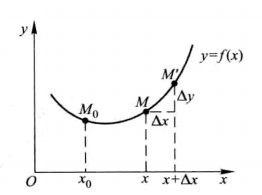
\includegraphics[width=.9\linewidth]{/media/wu/file/stuuudy/notes/images/miscellaneous/arc.png}
\end{center}
设函数\(f(x)\)在区间\((a,b)\)内具有连续导数,在曲线\(y=f(x)\)上取固定点
\(M_0(x_0,y_0)\)作为度量弧长的几点,并规定依\(x\)增大的方向作为曲线的争相,对
曲线上任一点\(M(x,y)\),规定有向弧度\(\arc{M_0M}\)的值\(s\)(简称为弧)如下:
\(s\)的绝对值的等于这弧段的长度,当有向弧段\(\arc{M_0M}\)的方向与曲线的正向一
致时,\(s>0\),相反时\(s<0\)

\begin{equation*}
\Delta s=\arc{M_0M'}-\arc{M_0M}=\arc{MM'}
\end{equation*}
于是
\begin{align*}
(\frac{\Delta s}{\Delta x})^2&=(\frac{\arc{MM'}}{\Delta x})^2=
(\frac{\arc{MM'}}{\abs{MM'}})^2\cdot\frac{\abs{MM'}^2}{(\Delta x)^2}\\
&=(\frac{\arc{MM'}}{\abs{MM'}})^2\cdot\frac{(\Delta x)^2+(\Delta y)^2}{(\Delta x)^2}\\
&=(\frac{\arc{MM'}}{\abs{MM'}})^2[1+(\frac{\Delta y}{\Delta x})^2]
\end{align*}
因此
\begin{equation*}
\frac{\Delta s}{\Delta x}=\pm\sqrt{(\frac{\arc{MM'}}{\abs{MM'}})^2\cdot[1+(\frac{\Delta y}{\Delta x})^2]}
\end{equation*}
令\(\Delta x\to0\)取极限,由于\(\Delta x\to0\)时,\(M'\to M\),这时弧的长度与弦的长度之
比的极限等于1,即
\begin{equation*}
\lim_{M'\to M}\frac{\abs{\arc{MM'}}}{\abs{MM'}}=1
\end{equation*}
又
\begin{equation*}
\lim_{\Delta x\to0}\frac{\Delta y}{\Delta x}=y'
\end{equation*}
因此
\begin{equation*}
\frac{ds}{dx}=\pm\sqrt{1+y'^2}
\end{equation*}
由于\(s=s(x)\)是单调增加函数,于是有
\begin{equation*}
ds=\sqrt{1+y'^2}dx
\end{equation*}

\begin{center}
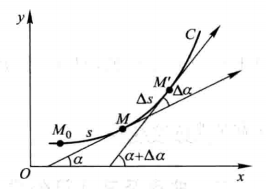
\includegraphics[width=.9\linewidth]{/media/wu/file/stuuudy/notes/images/miscellaneous/ArcDegree.png}
\end{center}

在曲线\(C\)上选定一点\(M_0\)作为度量弧\(s\)的基点,设曲线上点\(M\)对应与弧
\(s\),在点\(M\)处切线的倾角为\(\alpha\),曲线上另外一点\(M'\)对应于弧
\(s+\Delta s\),在点\(M'\)处切线的倾角为\(\alpha+\Delta \alpha\),则弧段
\(\arc{MM'}\)的长度为\(\abs{\Delta s}\)

我们用比值\(\abs{\frac{\Delta \alpha}{\Delta s}}\)来表达弧段\(\arc{MM'}\)的平均弯曲程度,叫
做弧段\(\arc{MM'}\)的 \textbf{平均曲率} ,并记作\(\bbar{K}\)

\begin{center}
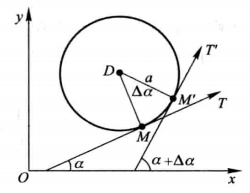
\includegraphics[width=.9\linewidth]{/media/wu/file/stuuudy/notes/images/miscellaneous/ArcCircle.png}
\end{center}

设圆的半径是\(a\),\(\angle MDM'=\frac{\Delta s}{a}\),因此
\begin{equation*}
\frac{\Delta\alpha}{\Delta s}=\frac{\frac{\Delta s}{a}}{\Delta s}=\frac{1}{a}
\end{equation*}
从而
\begin{equation*}
K=\abs{\frac{d\alpha}{d s}}=\frac{1}{a}
\end{equation*}

设曲线的直角坐标方程是\(y=f(x)\),且\(f(x)\)具有二阶导数,因为
\(\tan\alpha=y'\),所以
\begin{gather*}
\sec^2\alpha\frac{d\alpha}{dx}=y''\\
\frac{d\alpha}{dx}=\frac{y''}{1+\tan^2\alpha}=\frac{y''}{1+y'^2}
\end{gather*}
于是
\begin{equation*}
d\alpha=\frac{y''}{1+y'^2}dx
\end{equation*}
又因为
\begin{equation*}
ds=\sqrt{1+y'^2}dx
\end{equation*}
因此
\begin{equation*}
K=\frac{\abs{y''}}{(1+y'^2)^{3/2}}
\end{equation*}


\begin{center}
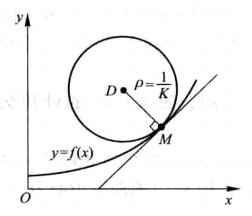
\includegraphics[width=.9\linewidth]{/media/wu/file/stuuudy/notes/images/miscellaneous/CurvatureCircle.png}
\end{center}
设曲线\(y=f(x)\)在点\(M(x,y)\)处的曲率为\(K(K\neq0)\),在点\(M\)处的曲线的法
线上,在凹的一侧取一点\(D\),使\(\abs{DM}=\frac{1}{K}=\rho\),以\(D\)为圆心,
\(\rho\) 为半径作圆,这个圆叫做曲线在点\(M\)处的 \textbf{曲率圆} ,\(D\)为 \textbf{曲率中心} , \(\rho\) 为曲
率半径
\section{不定积分}
\label{sec:orgebe77b0}
\section{Index}
\label{sec:org6707bf0}
\renewcommand{\indexname}{}
\printindex
\end{document}
